%%
%% This is file `thesis-test.tex',
%% generated with the docstrip utility.
%%
%% The original source files were:
%%
%% nuthesis.dtx  (with options: `thesis-test')
%% 

\documentclass[ms,testing]{nuthesis}
%% Needed to typset the math in this sample
\usepackage{amsmath}
\usepackage{amsfonts}
%% Let's use a different font
\usepackage[sc,osf]{mathpazo}

%% Makes things look better
\usepackage{microtype}

%% Makes things look better
\usepackage{booktabs}

%% Gives us extra list environments
\usepackage{paralist}

%% Be able to include graphicsx
\usepackage{graphicx}

%% I like darker colors
\usepackage{color}
\definecolor{dark-red}{rgb}{0.6,0,0}
\definecolor{dark-green}{rgb}{0,0.6,0}
\definecolor{dark-blue}{rgb}{0,0,0.6}

%% If you use hyperref, you need to load memhfixc *after* it.
%% See the memoir docs for details.
\usepackage[%
pdfauthor={James D. Duin},
pdftitle={Hierachical Active Learning Bioinformatics Application},
pdfsubject={BioDataset},
pdfkeywords={semi-supervised learning, active learning, hierarchical labeling, cost analysis},
linkcolor=dark-blue,
pagecolor=dark-green,
citecolor=dark-blue,
urlcolor=dark-red,
%colorlinks=true,
backref,
plainpages=false,% This helps to fix the issue with hyperref with page numbering
pdfpagelabels% This helps to fix the issue with hyperref with page numbering
]{hyperref}

%% Needed by memoir to fix things with hyperref
\usepackage{memhfixc}
\begin{document}
%% Start formating the first few special pages
%% frontmatter is needed to set the page numbering correctly
\frontmatter

\title{Hierachical Active Learning Bioinformatics Application}
\author{James D. Duin}
\adviser{Professor Stephen Scott}
\adviserAbstract{Stephen Scott}
\major{Computer Science}
\degreemonth{February}
\degreeyear{2017}
%%
%% For most people the defaults will be correct, so they are commented
%% out. To manually set these, just uncomment and make the needed
%% changes.
%% \college{Your college}
%% \city{Your City}
%%
%% For most people the following can be changed with a class
%% option. To manually set these, just uncomment the following and
%% make the needed changes.
%% \doctype{Thesis or Dissertation}
%% \degree{Your degree}
%% \degreeabbreviation{Your degree abbr.}
%%
%% Now that we know everything we need, we can generate the title page
%% itself.
%%
\maketitle
%% You have a maximum of 350, which includes your title, name, etc.
\begin{abstract}
  \par Many classification tasks target high-level concepts that can be
  decomposed into a hierarchy of finer-grained sub- concepts. For example,
  some string entities that are Locations are also Attractions, some Attractions
  are Museums, etc. Such hierarchies are common in named entity recognition (NER),
  document classification, and biological sequence analysis. We present a new approach
  for learning hierarchically decomposable concepts. The approach learns a high-level
  classifier (e.g., location vs. non-location) by seperately learning multiple
  finer-grained classifiers (e.g., museum vs. non-museum), and then combining the
  results. Soliciting labels at a finer level of granularity than that of the target
  concept is a new approach to active learning, which we term active over-labeling.
  In experiments in NER and document classification tasks, we show that active over-
  labeling substantially improves area under the precision-recall curve when compared
  with standard passive or active learning. Finally, because finer-grained labels may be
  more expensive to obtain, we also present a cost-sensitive active learner that uses a
  multi-armed bandit approach to dynamically choose the label granularity to target, and
  show that the bandit-based learner is robust to differences in label cost and labeling budget.
\end{abstract}

%% Optional
%\begin{copyrightpage}
%This file may be distributed and/or modified under the conditions of
%the \LaTeX{} Project Public License, either version 1.3c of this license
%or (at your option) any later version.  The latest version of this
%license is in:
%\begin{center}
%   \url{http://www.latex-project.org/lppl.txt}
%\end{center}
%and version 1.3c or later is part of all distributions of \LaTeX version
%2006/05/20 or later.
%\end{copyrightpage}

%% Optional
\begin{dedication}
  This thesis is dedicated to my parents Paul and Vicki Duin and fiancee Anna Spady.
\end{dedication}

%% Optional
\begin{acknowledgments}
  I would like to thank my advisor Dr. Stephen Scott, Yugi Mo, and Dr. Douglas Downey.
\end{acknowledgments}

%% Optional
%\begin{grantinfo}
%  I'm not funded by any grants.
%\end{grantinfo}
%%% The ToC is required
%%% Uncomment these if need be

%% The ToC is required
\tableofcontents
%% Uncomment these if need be
%\listoffigures
%\listoftables

%%   mainmatter is needed after the ToC, (LoF, and LoT) to set the
%%   page numbering correctly for the main body
\mainmatter

%% Thesis goes here
\chapter{Introduction}\label{chap:aenied}
\section{Machine Learning}
add text'example cite'\cite{Merialdo2001}
\subsection{Active Learning}
add text'example cite'\cite{Merialdo2001}
\subsubsection{Bio Informatics}
add text'example cite'\cite{Merialdo2001}







\chapter{Background and Related Work}
\section{Other Datasets from Yugi}
add text'example cite'\cite{Merialdo2001}
\section{Other Papers cited by Yugi}
add text'example cite'\cite{Merialdo2001}







\chapter{Bio HAL}\label{chap:math}
\section{Passive SVM Rbf kernel vs Logistic Reg}
add text'example cite'\cite{Merialdo2001}


\section{Active vs Passive curves}
\par The following plots were obtained with a round batch size of 100
and a starter set of 1040 instances out of the total 2098 instances.
The plots are the average of 10 folds, for each fold a test set of 2010
containing representatives of each class was held out, out of the remaining
18088, the starter set was selected which again contained representatives of
each class. Coarse and fine classifiers share the same starter set. During
 each round coarse and fine classifiers are trained on their corresponding
 sets, metrics are outputted on the held out test set, then confidence estimates
 are ran on the remaining eligible instances. Eligible instances are kept in
 separate sets for coarse and fine, 100 of the most uncertain instances are removed
 from each eligible set and added to its corresponding coarse or fine set to be
 trained on for the next round.

\subsection{Plots for Logistic Regression Active vs Passive curves}
\begin{figure}[!htb]
	\centering
    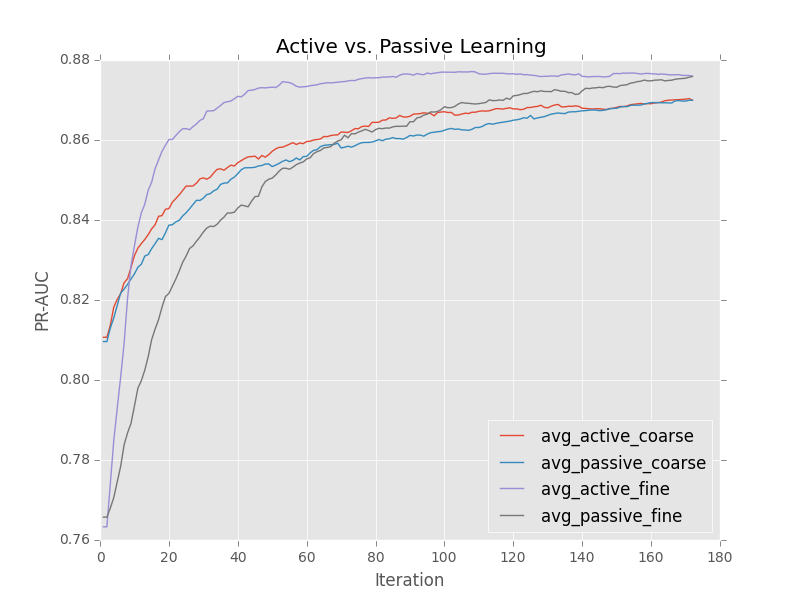
\includegraphics[width=\columnwidth]{fig/ActiveVsPassivePRLR}
    \label{fig:ActiveVsPassivePRLR}
    \caption{The PR AUC curves for rounds with the Logistic
Regression classifier conforms to expectations, with active-fine having
the highest performance. Active-coarse outperforms passive-coarse. Passive-fine
doesn't outperform the coarse classifiers until rnd 100. }
\end{figure}
\break
\begin{figure}[!htb]
	\centering
    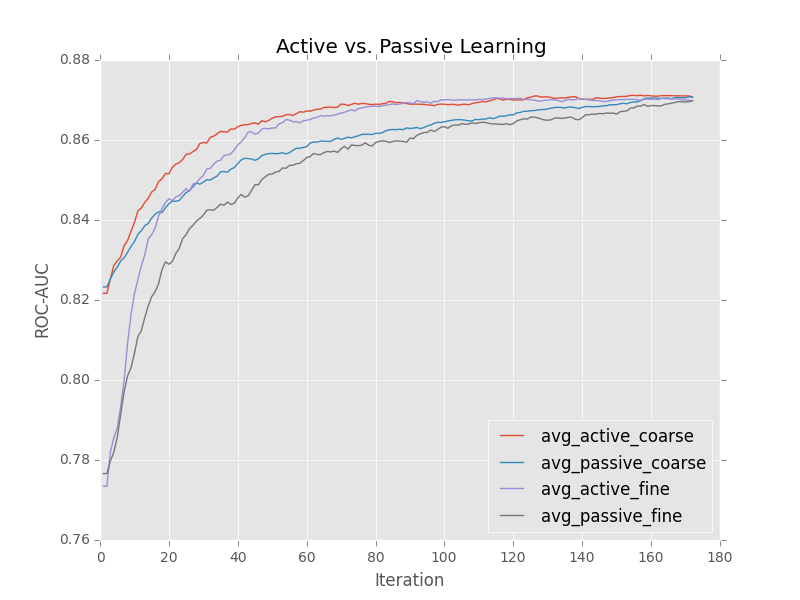
\includegraphics[width=\columnwidth]{fig/ActiveVsPassiveROCLR}
    \label{fig:ActiveVsPassiveROCLR}
    \caption{The ROC AUC curves for rounds with the
Logistic Regression classifier. The active curves beat out the passive
curves for both coarse and fine. Coarse roc starts with an advantage over
fine as in the PR curves. Both converge to the same rate after roc auc level after 80.}
\end{figure}
\break
\begin{figure}[!htb]
	\centering
    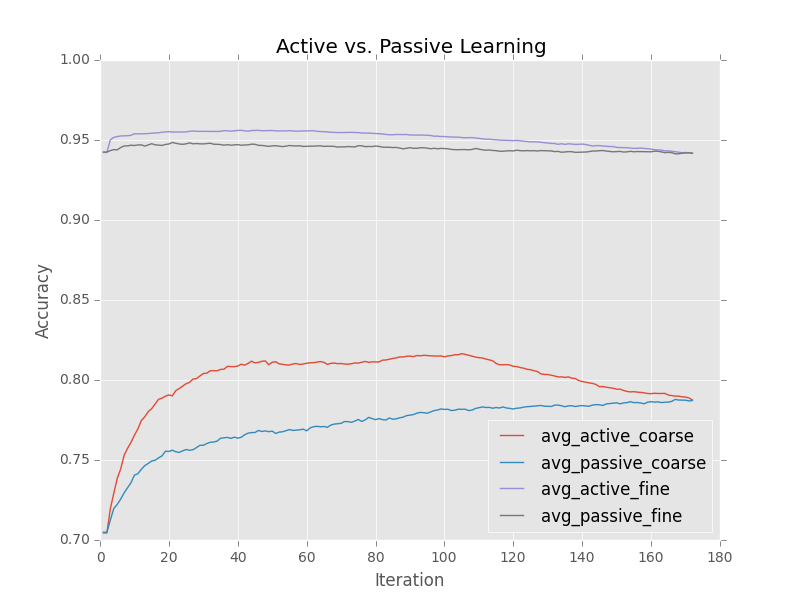
\includegraphics[width=\columnwidth]{fig/ActiveVsPassiveAccLR}
    \label{fig:ActiveVsPassiveAccLR}
    \caption{The accuracy of the fine classifiers stays at
roughly the same rate throughout the rounds, this is due to an effective
weighting scheme for the fine grained classifiers. The active coarse accuracy
drops towards the end due to an increase in false positives as more negative
instances are added in the later rounds.}
\end{figure}
\break
\begin{figure}[!htb]
	\centering
    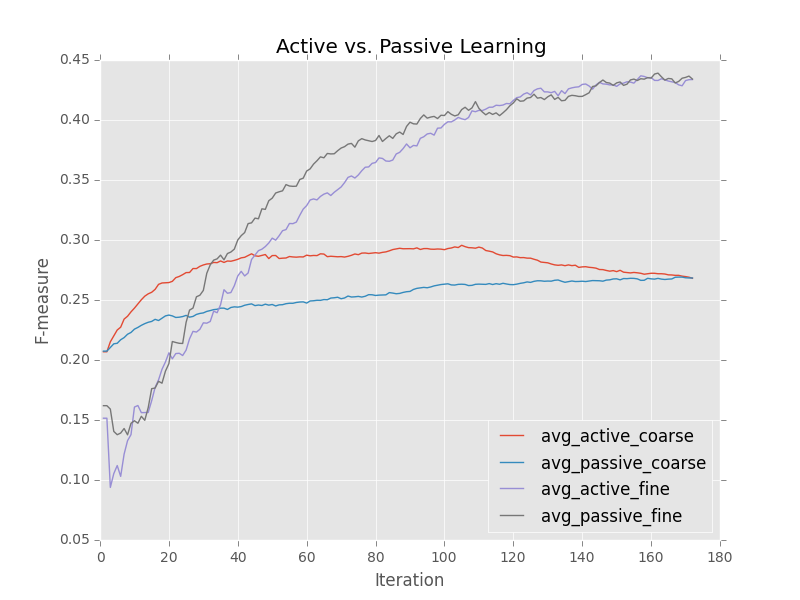
\includegraphics[width=\columnwidth]{fig/ActiveVsPassiveF1LR}
    \label{fig:ActiveVsPassiveF1LR}
    \caption{The F-measure of the the fine classifiers increases
throughout the rounds as more true positives are predicted. The active coarse
again decreases at later rounds due to increased false positives.}
\end{figure}
\break

\subsection{Plots for SVM Active vs Passive curves}
\begin{figure}[!htb]
	\centering
    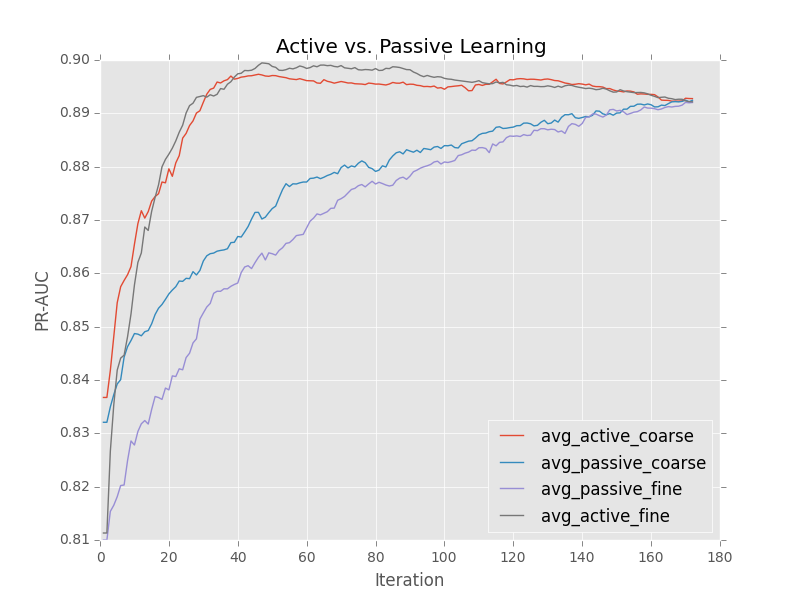
\includegraphics[width=\columnwidth]{fig/ActiveVsPassivePRSVM}
    \label{fig:ActiveVsPassivePRSVM}
    \caption{The PR AUC curves for rounds with SVM show little
advantage for fine. The results are slightly different than the ones shown
on 2/14 due to fixing a bug with the code that wasn't performing the
preprocessing scaling for the SVM case at the same stage as it was being
done for the logistic regression classifier.}
\end{figure}
\break
\begin{figure}[!htb]
	\centering
    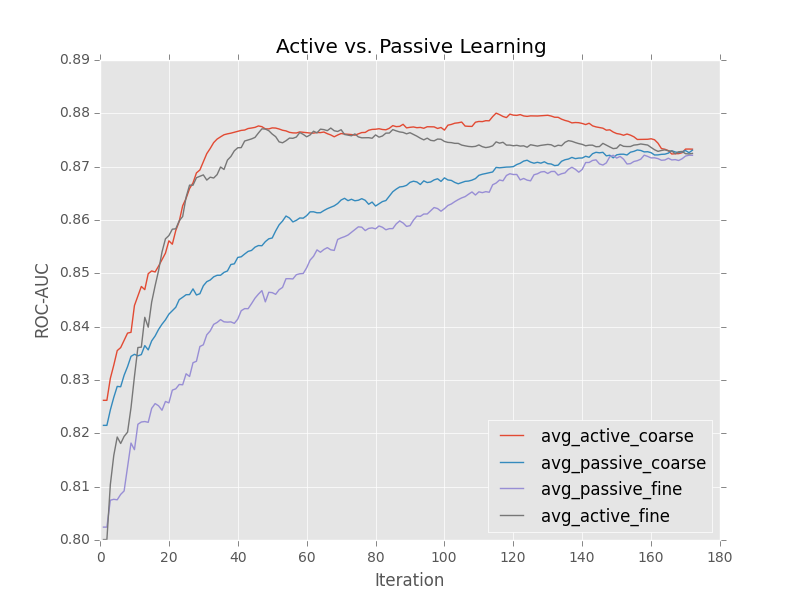
\includegraphics[width=\columnwidth]{fig/ActiveVsPassiveROCSVM}
    \label{fig:ActiveVsPassiveROCSVM}
    \caption{The ROC curves show more of an advantage for coarse classifiers.}
\end{figure}
\break
\begin{figure}[!htb]
	\centering
    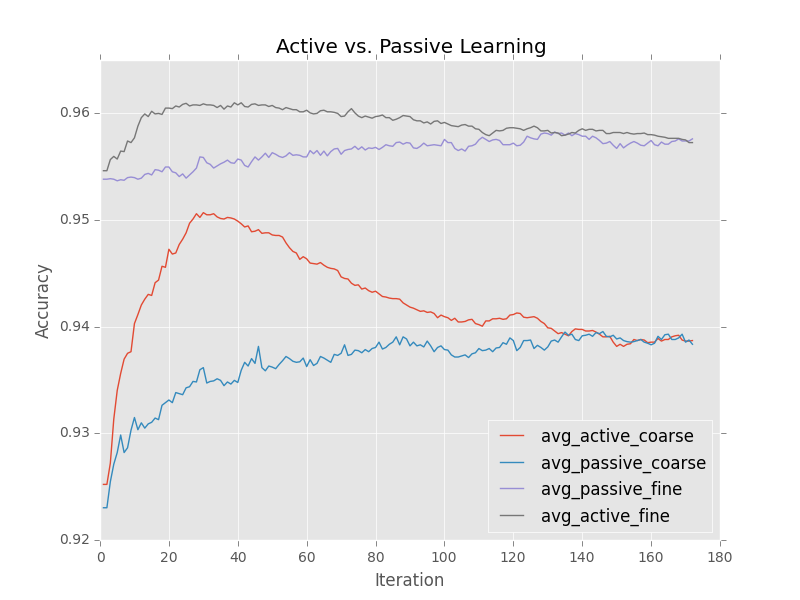
\includegraphics[width=\columnwidth]{fig/ActiveVsPassiveAccSVM}
    \label{fig:ActiveVsPassiveAccSVM}
    \caption{The accuracy for the coarse decreases sharply due
to coarse predicting steadily more false positives, behaving similar to the
Log Reg case. Fine accuracy is higher due to predicting less false positives
than coarse. Fine also predicts less true positives, compare apx. 37 to apx.
60 t.p. for coarse at round 60.}
\end{figure}
\break
\begin{figure}[!htb]
	\centering
    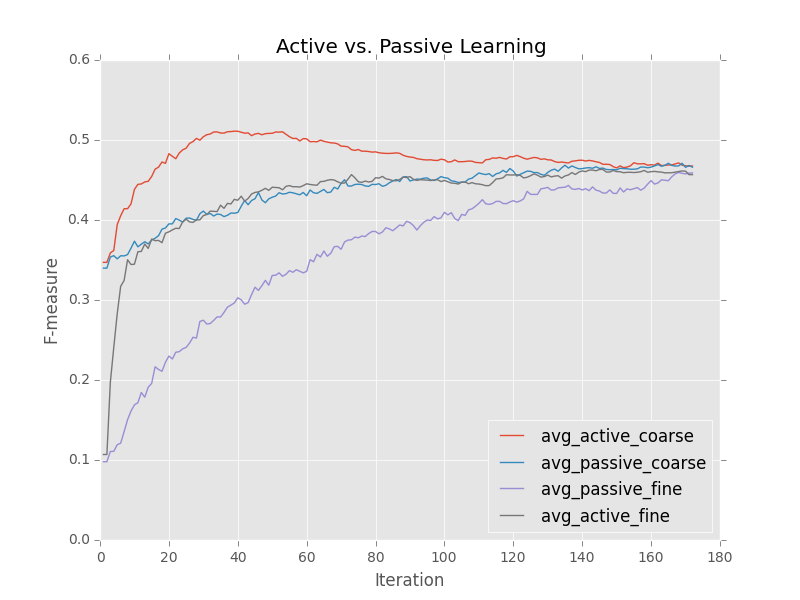
\includegraphics[width=\columnwidth]{fig/ActiveVsPassiveF1SVM}
    \label{fig:ActiveVsPassiveF1SVM}
    \caption{The F-measure favors coarse, and trends to the same level
    for both coarse and fine.}
\end{figure}
\break

\section{Plots for FFR experiments}
\begin{figure}[!htb]
	\centering
    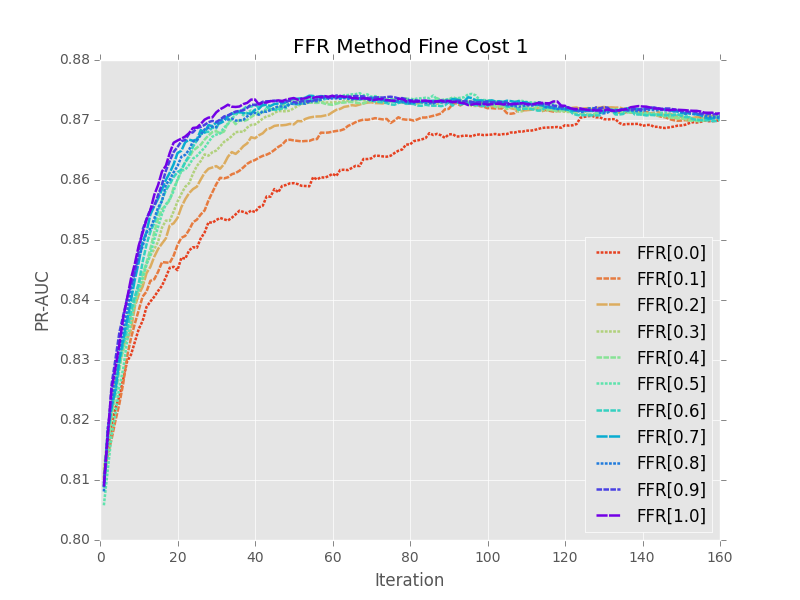
\includegraphics[width=\columnwidth]{fig/FFR_PR_Cost1}
    \label{fig:FFR_PR_Cost1}
    \caption{The round size is changed to 160 and a fine has a cost of 1.
The 0p5 round for instance, corresponds to 0.5 of the total budget being used on fine,
so 80 goes to fine and 80 goes to coarse. For the 0p0 round, none of the budget is
used for fine and it has the worst performance. After around 0p3 the gains in performance
are marginal. The performance increases with the green 1p0 curve outperforming the
rest. The results are an average of 10 folds.}
\end{figure}
\break
\begin{figure}[!htb]
	\centering
    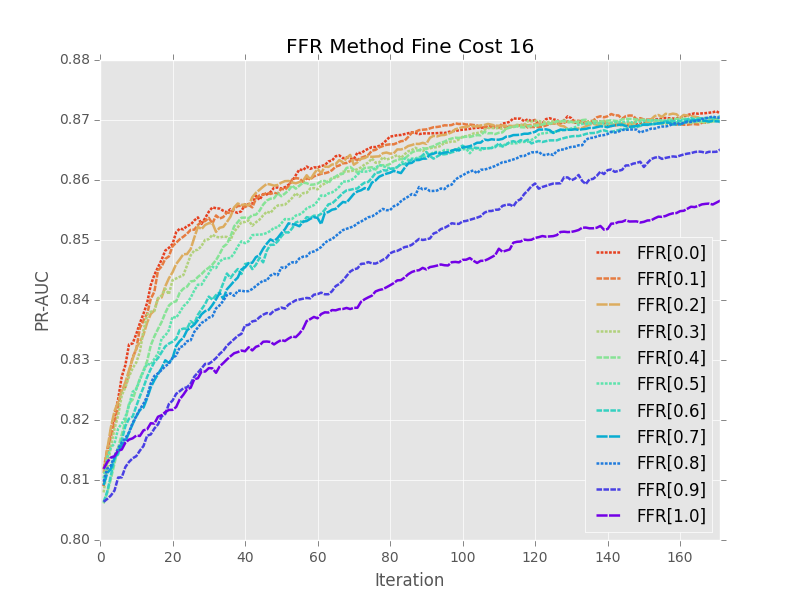
\includegraphics[width=\columnwidth]{fig/FFR_PR_Cost16}
    \label{fig:FFR_PR_Cost16}
    \caption{The round size is again 160 and fine has a cost of 16. The worst
    performing curve is again 0p0 with no fine instances, but the benefit of fine
    instances is marginal. For the 0p5 case 5 instances are purchased for fine and
    80 are purchased for coarse. For the 1p0 case 16 instances are purchase for
    fine and 144 instances are purchased for coarse.}
\end{figure}
\break






\chapter{Conclusions and Future Work}\label{chap:math}
\par add text'example cite'\cite{Merialdo2001}










%% backmatter is needed at the end of the main body of your thesis to
%% set up page numbering correctly for the remainder of the thesis
\backmatter

%% Start the correct formatting for the appendices
\appendix

\chapter{Tuning the fine grained classes}
\par add text'example cite'\cite{Merialdo2001}

%% Bibliography goes here (You better have one)
%% BibTeX is your friend
\bibliographystyle{plain}
\bibliography{nuthesis}
%% Pull in all the entries in the bibtex file. Is is a useful trick to
%% check all your references.
\nocite{*}


%% Index go here (if you have one)

\end{document}
\endinput
%%
%% End of file `thesis-test.tex'.
